% Frames

% Rewriting => Giv et overview over de tools, konkret eksempel paa hvordan man implementerer det i et af tools'ene, kig paa hvilke features der er i hvert tool og stil det mere systematisk op end i rapporten

\begin{frame}{Annotate Bytecode}{}
\begin{itemize}
\item When does a fault compromise the code?
\item What is a sensitive region and how do we determine a successful run?
\item What about variable inputs? 
\end{itemize}
%\textit{figure to the left with critical region not defined}
\end{frame}
%focused security, selectiv

\begin{frame}[fragile]{Annotate Bytecode}{}
\begin{minipage}{.30\textwidth}
\begin{itemize}
\item Parameter set.
\item Assessments
\end{itemize}

\end{minipage}%
\hspace{20px}
\begin{minipage}{0.60\textwidth}
\begin{lstlisting}[frame=single]
public int stub()
 0: push 7  //*VALID(1,3,5)
 	          //*INVALID(2,4)
 2: ireturn 

...
 4: ifeq 9
 7: aload_5 
 8: athrow
 9: aload_0  //*ASSERT VALID
...
\end{lstlisting}
\end{minipage}
\end{frame}

\begin{frame}[fragile]{UPPAAL Representation}{Virtual}


\begin{lstlisting}[frame=single]
public int foo() { return bar() + 1; }
public int bar() { return 4; }
\end{lstlisting}

\begin{figure}
\centering
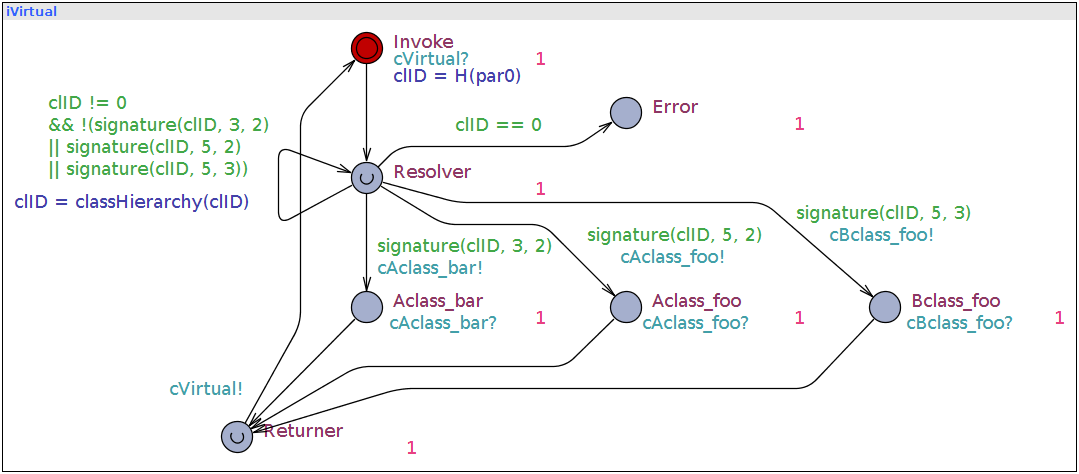
\includegraphics[width=0.8\textwidth]{figures/oldvirtual.png}
\caption{\footnotesize Virtual template as it apears in the virtual example}
\end{figure}
\end{frame}

\begin{frame}[fragile]{Representation}{Virtual}
\begin{figure}
\centering
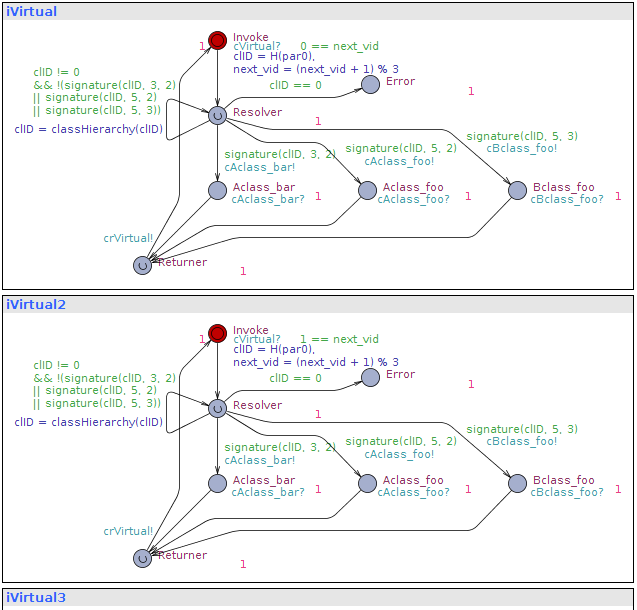
\includegraphics[width=0.6\textwidth]{figures/newVirtual.png}
\caption{\footnotesize A virtual template foreach virtual method.}
\end{figure}
\end{frame}

\begin{frame}{Representation}{}
\begin{block}{Possible solution: Single template for all methods.}
\begin{itemize}
\item Remove waiting locations.
\item Replace all channel synchronisation with edges for method calls.
\item Make a representation for the Call Stack.
\end{itemize}

\end{block}
\end{frame}


\begin{frame}{Full Automation}{}
\begin{itemize}
\item UPPAAL CLI
\end{itemize}
\textit{figure of cli}
\end{frame}

\begin{frame}{Demo}{}
example.
\end{frame}

